\documentclass[10pt, hyperref={unicode}]{beamer}

\usepackage{times}
\usepackage[czech]{babel}
\usepackage[utf8]{inputenc}
\usepackage{graphics} 
\usepackage{booktabs} 
\usepackage{listings} 
\usepackage{xcolor} 
\usepackage[ruled, czech, linesnumbered, noline, longend]{algorithm2e}
\usepackage{graphicx}
\usepackage{amssymb}
\usepackage{amsmath}
\usepackage{amsthm}

\usetheme{Warsaw}

\setbeamertemplate{footline}[frame number]

\definecolor{commentgray}{RGB}{150,150,150}
\definecolor{keywordpurple}{RGB}{170,30,70}
\definecolor{stringblue}{RGB}{20,50,120}

\lstset{
	basicstyle=\footnotesize,
	commentstyle=\color{commentgray},
	frame=single,
	keepspaces=true,
	keywordstyle=\color{keywordpurple},
	language=C,
	morekeywords={new, use},
	numbers=left,
	stringstyle=\color{stringblue},
	showstringspaces=false,
	showspaces=false,
	showtabs=false,
	tabsize=4,
}

\setbeamertemplate{footline}[frame number]

\title{Typografie a~publikování\,--\,5.~projekt}
\subtitle{Bubble Sort}
\author{Maroš Geffert\texorpdfstring{\\ xgeffe00@stud.fit.vutbr.cz}{}}
\date{\today}
\institute
{
	Vysoké učení technické v~Brně\\
	Fakulta informačních technologií
}

\begin{document}

\maketitle

\section{Představení bubble sortu}

\begin{frame}{Bubble sort}
	\begin{itemize}
		\item
		    \alert{Bubble sort} je implementačně jednoduchý řadicí algoritmus.
		    \pause
		\item
			Algoritmus je: 
			\begin{itemize}
			    \pause
				\item Univerzální \textit{(pracuje na~základě porovnávání dvojic prvků).}
				\pause
				\item Pracuje lokálně \textit{(nevyžaduje pomocnou paměť).}
				\pause
				\item Je stabilní \textit{(prvkům se stejným klíčem nemění vzájemnou polohu).}
				\pause
				\item Tento řadíci algoritmus je jedným z~najpomalejších
				\pause
				\item Algoritmus probíhá ve~vlnách, přičemž při~každé vlně propadne "nejtěžší" prvek na~konec
			\end{itemize}
	\end{itemize}
\end{frame}


\begin{frame}{Využití}
	\begin{itemize}
		\item
			Algoritmus opakovaně prochází seznam, přičemž porovnává každé dva sousedící prvky, a pokud nejsou ve~správném pořadí, prohodí je. 
		\item	
			Využívá se hlavně pro~výukové účely či v~nenáročných aplikacích. 
			\begin{enumerate}
				\item Název vyjadřuje průběh zpracování, při~kterém prvky s~vyšší hodnotou „probublávají“ na~konec seznamu. 
				\item Optimalizací algoritmu je detekce prohození prvků v~průchodu seznamu. 
			\end{enumerate}

		\item
			V~případě, že algoritmus v~průchodu neprohodil žádné dva prvky, řazení můžeme ukončit s~tím, že seznam je seřazen. 
	\end{itemize}
\end{frame}


\section{Algoritmy bubble sortu}

\begin{frame}[fragile]{Algoritmy bubble sortu}
	\begin{alertblock}{\texttt{Algoritmus}}
		\begin{itemize}
			\item Poznámka: toto je jen jedna z~mnoha variací algoritmu. 
		\end{itemize}
	\end{alertblock}

\begin{lstlisting}
opakuj
    bylo_serazeno := true;
    for i from 1 to (pocet_prvku - 1) opakuj:
        pokud seznam[i] > seznam[i + 1]
            zamen(seznam[i], seznam[i + 1])
            bylo_serazeno := false;
dokud neni bylo_serazeno == true;
\end{lstlisting}
\end{frame}

\begin{frame}[fragile]{Alternativní verze bubble sortu}
	\begin{alertblock}{\texttt{Alternativní verze}}
		\begin{itemize}
			\item Výhodou alternativní verze je o~něco vyšší efektivita. 
			\item Po $n$ opakováních je spodních $n$ prvků již seřazeno a je zbytečné je znovu procházet. 
			\item Další výhodou je, že upravený algoritmus se nezacyklí v~nekonečné smyčce ani v~případě, že bychom měli špatně implementovanou funkci pro~porovnávání prvků seznamu. 
		\end{itemize}
	\end{alertblock}

\begin{lstlisting}
limit := pocet_prvku;
opakuj
    bylo_serazeno := true;
    limit := limit - 1;
    for i from 1 to limit opakuj:
        pokud seznam[i] > seznam[i + 1]
            zamen(seznam[i], seznam[i + 1])
            bylo_serazeno := false;
dokud neni bylo_serazeno == true or limit == 1;
\end{lstlisting}
\end{frame}

\begin{frame}[fragile]{Příklad bubble sortu v~jazyku C}

\begin{lstlisting}
// Funkce na implementaci bubble sortu
void bubbleSort(int arr[], int n) 
{ 
   int i, j; 
   for (i = 0; i < n-1; i++)       
  
       // posledni i elementy sou na miste
       for (j = 0; j < n-i-1; j++)  
           if (arr[j] > arr[j+1]) 
              swap(&arr[j], &arr[j+1]); 
} 
\end{lstlisting}
\end{frame}

\section{Výhody a nevýhody bubble sortu}

\begin{frame}{Výhody}
	\begin{itemize}
		\item
			Bubble sort je z~hlediska naprogramování nejjednodušším algoritmem pro~řazení.
		\item	
			Výhodou rovněž je, že je stabilní, \textit{(tzn. nemění pozici prvků)}, které jsou při~porovnávání vyhodnoceny jako ekvivalentní. 
		\item
		    Bublinkové řazení je jeden z~mála řadicích algoritmů, kterému stačí sekvenční přístup k~datům
		\item
		    V~minulosti se proto používal k~řazení dat na~páskových médiích, dnes jej lze s~výhodou použít například při~řazení jednosměrně zřetězeného spojového seznamu. 
	\end{itemize}
\end{frame}

\begin{frame}[fragile]{Nevýhody}
	\begin{alertblock}{{}}
		\begin{itemize}
			\item Pro~řazení opravdu velkých polí je bublinkové řazení naprosto \textbf{nevhodné}.
			\item Pokud např. seřazení desetiprvkového pole trvá jednotku času, pak při~bubble sortu stokrát delšího (tisíciprvkového pole) spotřebujeme 10000 jednotek času, zatímco kvalitní algoritmus by potřeboval pouze 200 jednotek času.
			\item Další nevýhodou jsou zbytečná porovnání při~řazení seznamu s~nejnižším prvkem na~konci.
			\item Nepomůže ani optimalizace pomocí detekce prohození prvků, jelikož tento nejnižší prvek se v~každém průchodu posune o~jedno místo vlevo. \textit{(Tento problém řeší modifikace algoritmu nazvaná Shaker sort).} 
		\end{itemize}
	\end{alertblock}
\end{frame}

\section{Časová složitost}
\begin{frame}{Časová složitost}

			\begin{itemize}
				\item Průměrná i nejhorší asymptotická složitost bubble sortu je $O(n^2)$. 
			\end{itemize}
			
			\begin{figure}[h]
                 \centering
                     \scalebox{0.4}{
                         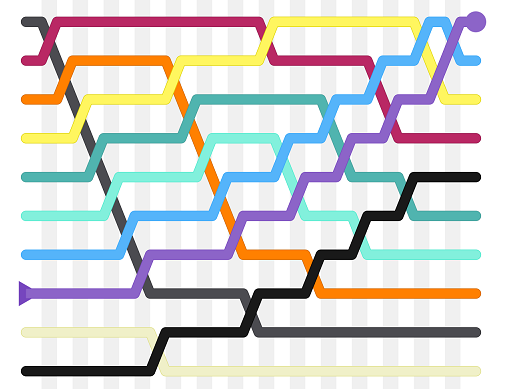
\includegraphics{obr1.png}
                         }
               \caption{Barpngý diagram bubble sortu - barva označuje prvek řazené posloupnosti, zleva doprava sledujeme možný průběh řazení.}
\end{figure}

\end{frame}



\begin{frame}{Použité zdroje}
	\begin{thebibliography}{10}
		\bibitem[Bubble Sort]{bubble} Bubble Sort
		\newblock \texttt{https://www.geeksforgeeks.org/bubble-sort/}
		\bibitem[Bubble Sort, ITnetwork.cz]{bubble} ITnetwork.cz: Bubble Sort
		\newblock \texttt{https://www.itnetwork.cz/navrh/algoritmy/algoritmy-razeni/algoritmus-bubblesort-probublavani-trideni-cisel/}
		\bibitem[Bubble Sort]{bubble} Bubble Sort
		\newblock \texttt{http://www.zbynek.adamh.cz/cs/02066/Programovani/Clanky/Razeni-metodou-bubble-sort/}
	\end{thebibliography}
\end{frame}

\end{document}
